%\clearpage
\section{Background Estimation Techniques}
\label{sec:bkg}

In this section we describe the techniques used to estimate the SM backgrounds in our signal regions defined by requirements of large \MET.
The SM backgrounds fall into three categories:

\begin{itemize}
\item \zjets: this is the dominant background after the preselection. The \MET\ in \zjets\ events is estimated with the 
``\MET\ templates'' technique described in Sec.~\ref{sec:bkg_zjets};
\item Flavor-symmetric (FS) backgrounds: this category includes processes which produces 2 leptons of uncorrelated flavor. It is dominated
by \ttbar\ but also contains Z$\to\tau\tau$, WW, and single top processes. This is the dominant contribution in the signal regions, and it
is estimated using a data control sample of e$\mu$ events as described in Sec.~\ref{sec:bkg_fs};
\item WZ and ZZ backgrounds: this background is estimated from MC, after validating the MC modeling of these processes using data control
samples with jets and exactly 3 leptons (WZ control sample) and exactly 4 leptons (ZZ control sample) as described in Sec.~\ref{sec:bkg_vz};
%\item Rare SM backgrounds: this background contains rare processes such as $t\bar{t}$V and triple vector boson processes VVV (V=W,Z).
%This background is estimated from MC as described in Sec.~\ref{sec:bkg_raresm}. {\bf FIXME: add rare MC}
\end{itemize}

\subsection{Estimating the \zjets\ Background with \MET\ Templates}
\label{sec:bkg_zjets}

The premise of this data driven technique is that \MET\ in \zjets\ events
is produced by the hadronic recoil system and {\it not} by the leptons making up the Z.
Therefore, the basic idea of the \MET\ template method is to measure the \MET\ distribution in 
a control sample which has no true MET and the same general attributes regarding
fake MET as in \zjets\ events. We thus use a sample of \gjets\ events, since both \zjets\
and \gjets\ events consist of a well-measured object recoiling against hadronic jets.

For selecting photon-like objects, the very loose photon selection described in Sec.~\ref{sec:phosel} is used.
It is not essential for the photon sample to have high purity. For our purposes, selecting jets with predominantly 
electromagnetic energy deposition in a good fiducial volume suffices to ensure that 
they are well measured and do not contribute to fake \MET. The \gjets\ events are selected with a suite of
single photon triggers with \pt thresholds varying from 22--90 GeV. The events are weighted by the trigger prescale
such that \gjets\ events evenly sample the conditions over the full period of data taking.
There remains a small difference in the PU conditions in the \gjets\ vs. \zjets\ samples due to the different
dependencies of the $\gamma$ vs. Z isolation efficiencies on PU. To account for this, we reweight the \gjets\ samples
to match the distribution of reconstructed primary vertices in the \zjets\ sample.

To account for kinematic differences between the hadronic systems in the control vs. signal 
samples, we measure the \MET\ distributions in the \gjets\ sample in bins of the number of jets 
and the scalar sum of jet transverse energies (\Ht). These \MET\ templates are extracted separately from the 5 single photon
triggers with thresholds 22, 36, 50, 75, and 90 GeV, so that the templates are effectively binned in photon \pt.
All \MET distributions are normalized to unit area to form ``MET templates''.
The prediction of the MET in each \Z event is the template which corresponds to the \njets,
\Ht, and Z \pt in the \zjets\ event. The prediction for the \Z sample is simply the sum of all such templates.
All templates are displayed in App.~\ref{app:templates}.

While there is in principle a small contribution from backgrounds other than \zjets\ in the preselection regions,
this contribution is only $\approx$3\% ($\approx$2\%) of the total sample in the inclusive search (targeted search),
as shown in Table~\ref{table:zyields_2j} (Table~\ref{table:zyields_2j_targeted}), and is therefore negligible compared to the total 
background uncertainty.

\subsection{Estimating the Flavor-Symmetric Background with e$\mu$ Events}
\label{sec:bkg_fs}

In this subsection we describe the background estimate for the FS background. Since this background produces equal rates of same-flavor (SF)
ee and $\mu\mu$ lepton pairs as opposite-flavor (OF) e$\mu$ lepton pairs, the OF yield can be used to estimate the SF yield, after
correcting for the different electron vs. muon offline selection efficiencies and the different efficiencies for the ee, $\mu\mu$, and e$\mu$ triggers.

An important quantity needed to translate from the OF yield to a prediction for the background in the SF final state is the ratio 
$R_{\mu e} = \epsilon_\mu / \epsilon_e$, where $\epsilon_\mu$ ($\epsilon_e$) indicates the offline muon (electron) selection efficiency. 
This quantity can be extracted from data using the observed Z$\to\mu\mu$ and Z$\to$ee yields in the preselection region, after correcting 
for the different trigger efficiencies.

Hence we define:

\begin{itemize}
\item $N_{ee}^{\rm{trig}} = \epsilon_{ee}^{\rm{trig}}N_{ee}^{\rm{offline}}$,
\item $N_{\mu\mu}^{\rm{trig}} = \epsilon_{\mu\mu}^{\rm{trig}}N_{\mu\mu}^{\rm{offline}}$,
\item $N_{e\mu}^{\rm{trig}} = \epsilon_{e\mu}^{\rm{trig}}N_{e\mu}^{\rm{offline}}$.
\end{itemize}
 
Here $N_{\ell\ell}^{\rm{trig}}$ denotes the number of selected Z events in the $\ell\ell$ channel passing the offline and trigger selection
(in other words, the number of recorded and selected events), $\epsilon_{\ell\ell}^{\rm{trig}}$ is the trigger efficiency, and 
$N_{\ell\ell}^{\rm{offline}}$ is the number of events that would have passed the offline selection if the trigger had an efficiency of 100\%.
Thus we calculate the quantity:

\begin{equation}
R_{\mu e} = \sqrt{\frac{N_{\mu\mu}^{\rm{offline}}}{N_{ee}^{\rm{offline}}}} = \sqrt{\frac{N_{\mu\mu}^{\rm{trig}}/\epsilon_{\mu\mu}^{\rm{trig}}}{N_{ee}^{\rm{trig}}/\epsilon_{ee}^{\rm{trig}}}} 
= \sqrt{\frac{80367/0.88}{54426/0.95}} = 1.26\pm0.07.
\end{equation}

Here we have used the Z$\to\mu\mu$ and Z$\to$ee yields from Table~\ref{table:zyields_2j} and the trigger efficiencies quoted in Sec.~\ref{sec:datasets}.
The indicated uncertainty is due to the 3\% uncertainties in the trigger efficiencies. %{\bf FIXME: check for variation w.r.t. lepton \pt}.
The predicted yields in the ee and $\mu\mu$ final states are calculated from the observed e$\mu$ yield as

\begin{itemize}
\item $N_{ee}^{\rm{predicted}}    = \frac {N_{e\mu}^{\rm{trig}}} {\epsilon_{e\mu}^{\rm{trig}}} \frac {\epsilon_{ee}^{\rm{trig}}} {2 R_{\mu e}} 
= \frac{N_{e\mu}^{\rm{trig}}}{0.92}\frac{0.95}{2\times1.26} = (0.41\pm0.05) \times N_{e\mu}^{\rm{trig}}$ ,
\item $N_{\mu\mu}^{\rm{predicted}} = \frac {N_{e\mu}^{\rm{trig}}} {\epsilon_{e\mu}^{\rm{trig}}} \frac {\epsilon_{\mu\mu}^{\rm{trig}} R_{\mu e}}  {2}
= \frac {N_{e\mu}^{\rm{trig}}} {0.95} \frac {0.88 \times 1.26}{2} = (0.58\pm0.07) \times N_{e\mu}^{\rm{trig}}$,
\end{itemize}

and the predicted yield in the combined ee and $\mu\mu$ channel is simply the sum of these two predictions:

\begin{itemize}
\item $N_{ee+\mu\mu}^{\rm{predicted}} = (0.99\pm0.06)\times N_{e\mu}^{\rm{trig}}$.
\end{itemize}

Note that the relative uncertainty in the combined ee and $\mu\mu$ prediction is smaller than those for the individual ee and $\mu\mu$ predictions
because the uncertainty in $R_{\mu e}$ cancels when summing the ee and $\mu\mu$ predictions. %{\bf N.B. these uncertainties are preliminary}.

To improve the statistical precision of the FS background estimate, we remove the requirement that the e$\mu$ lepton pair falls in the Z mass window.
Instead we scale the e$\mu$ yield by $K$, the efficiency for e$\mu$ events to satisfy the Z mass requirement, extracted from simulation. In Fig.~\ref{fig:K_incl}
we display the value of $K$ in data and simulation, for a variety of \MET\ requirements, for the inclusive analysis. Based on this we chose $K=0.14\pm0.02$
for all \MET\ regions except for \MET\ $>$ 300 GeV. For this region the statistical precision is reduced, so that we inflate the uncertainty and chose $K=0.14\pm0.08$.
The corresponding plot for the targeted analysis, including the b-veto, is displayed in Fig.~\ref{fig:K_targeted}.
Based on this we chose $K=0.13\pm0.02$
for all \MET\ regions up to  \MET\ $>$ 100 GeV. For higher \MET\ regions (\MET\ $>$ 150 GeV and above) the statistical precision is reduced, 
so that we inflate the uncertainty and chose $K=0.13\pm0.07$.

\begin{figure}[!ht]
\begin{center}
\begin{tabular}{cc}
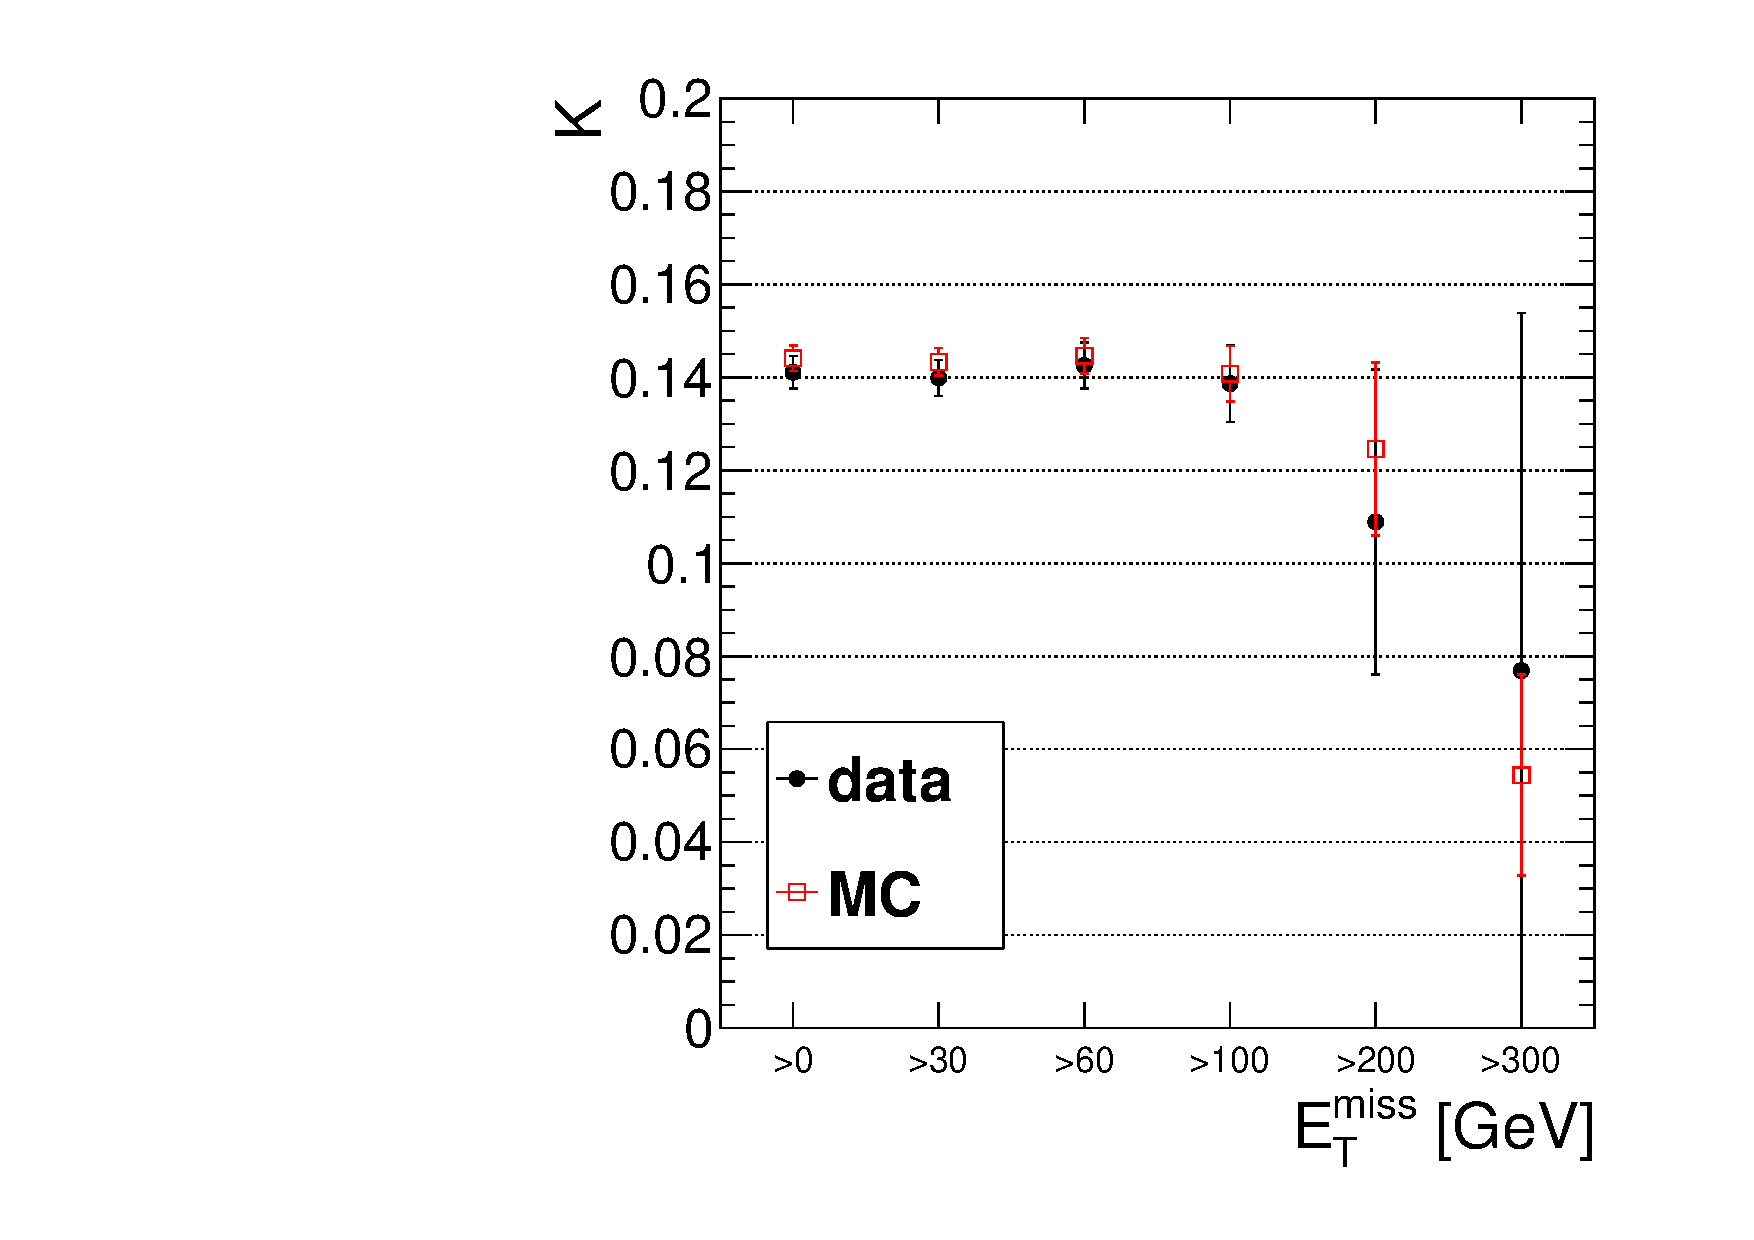
\includegraphics[width=0.4\textwidth]{plots/K_incl.pdf} &
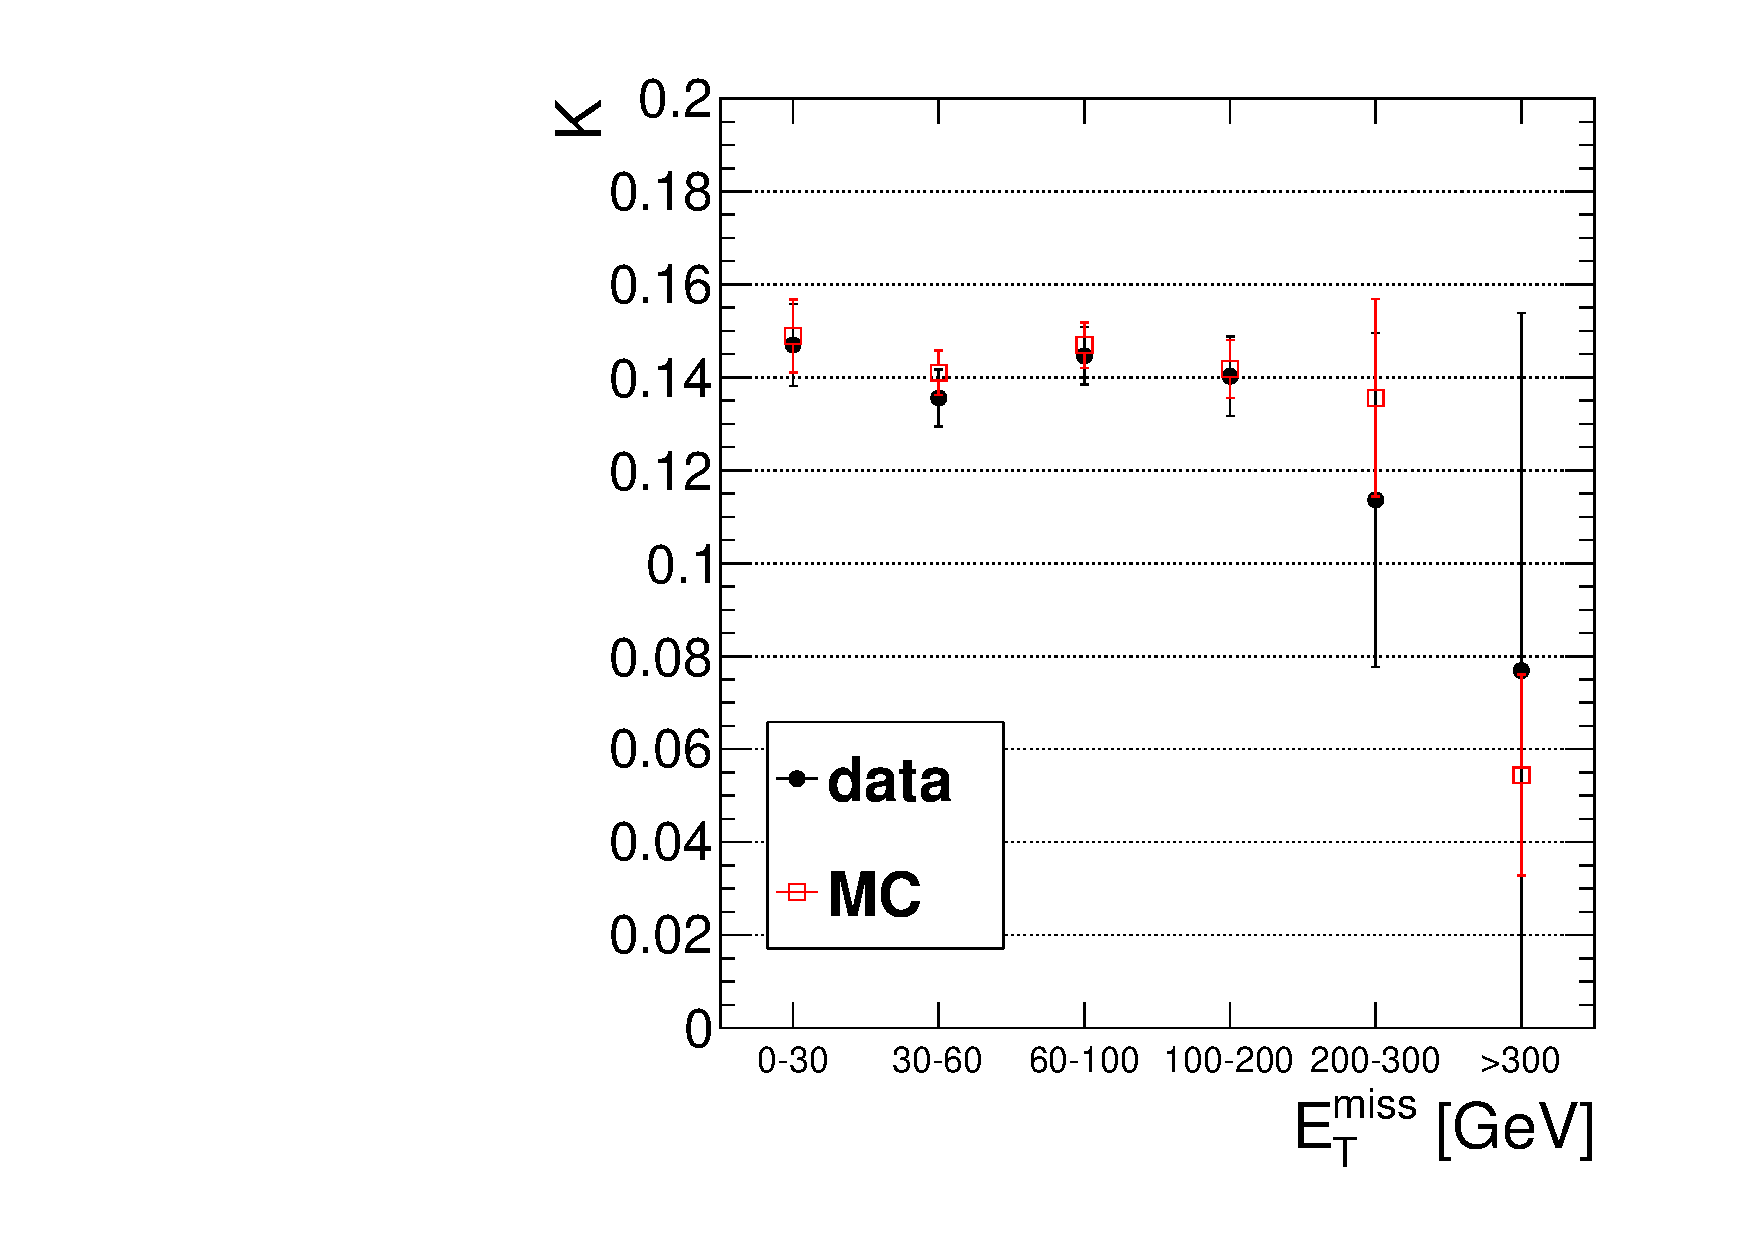
\includegraphics[width=0.4\textwidth]{plots/K_excl.pdf} \\
\end{tabular}
\caption{
The efficiency for e$\mu$ events to satisfy the dilepton mass requirement, $K$, in data and simulation for inclusive \MET\ intervals (left) and
exclusive \MET\ intervals (right) for the inclusive analysis. Based on this we chose $K=0.14\pm0.02$ for all \MET\ regions except \MET\ $>$ 300 GeV,
where we chose $K=0.14\pm0.08$.
%{\bf FIXME plots made with 10\% of \zjets\ MC statistics, to be remade with full statistics}
\label{fig:K_incl}
}
\end{center}
\end{figure}

\begin{figure}[!hb]
\begin{center}
\begin{tabular}{cc}
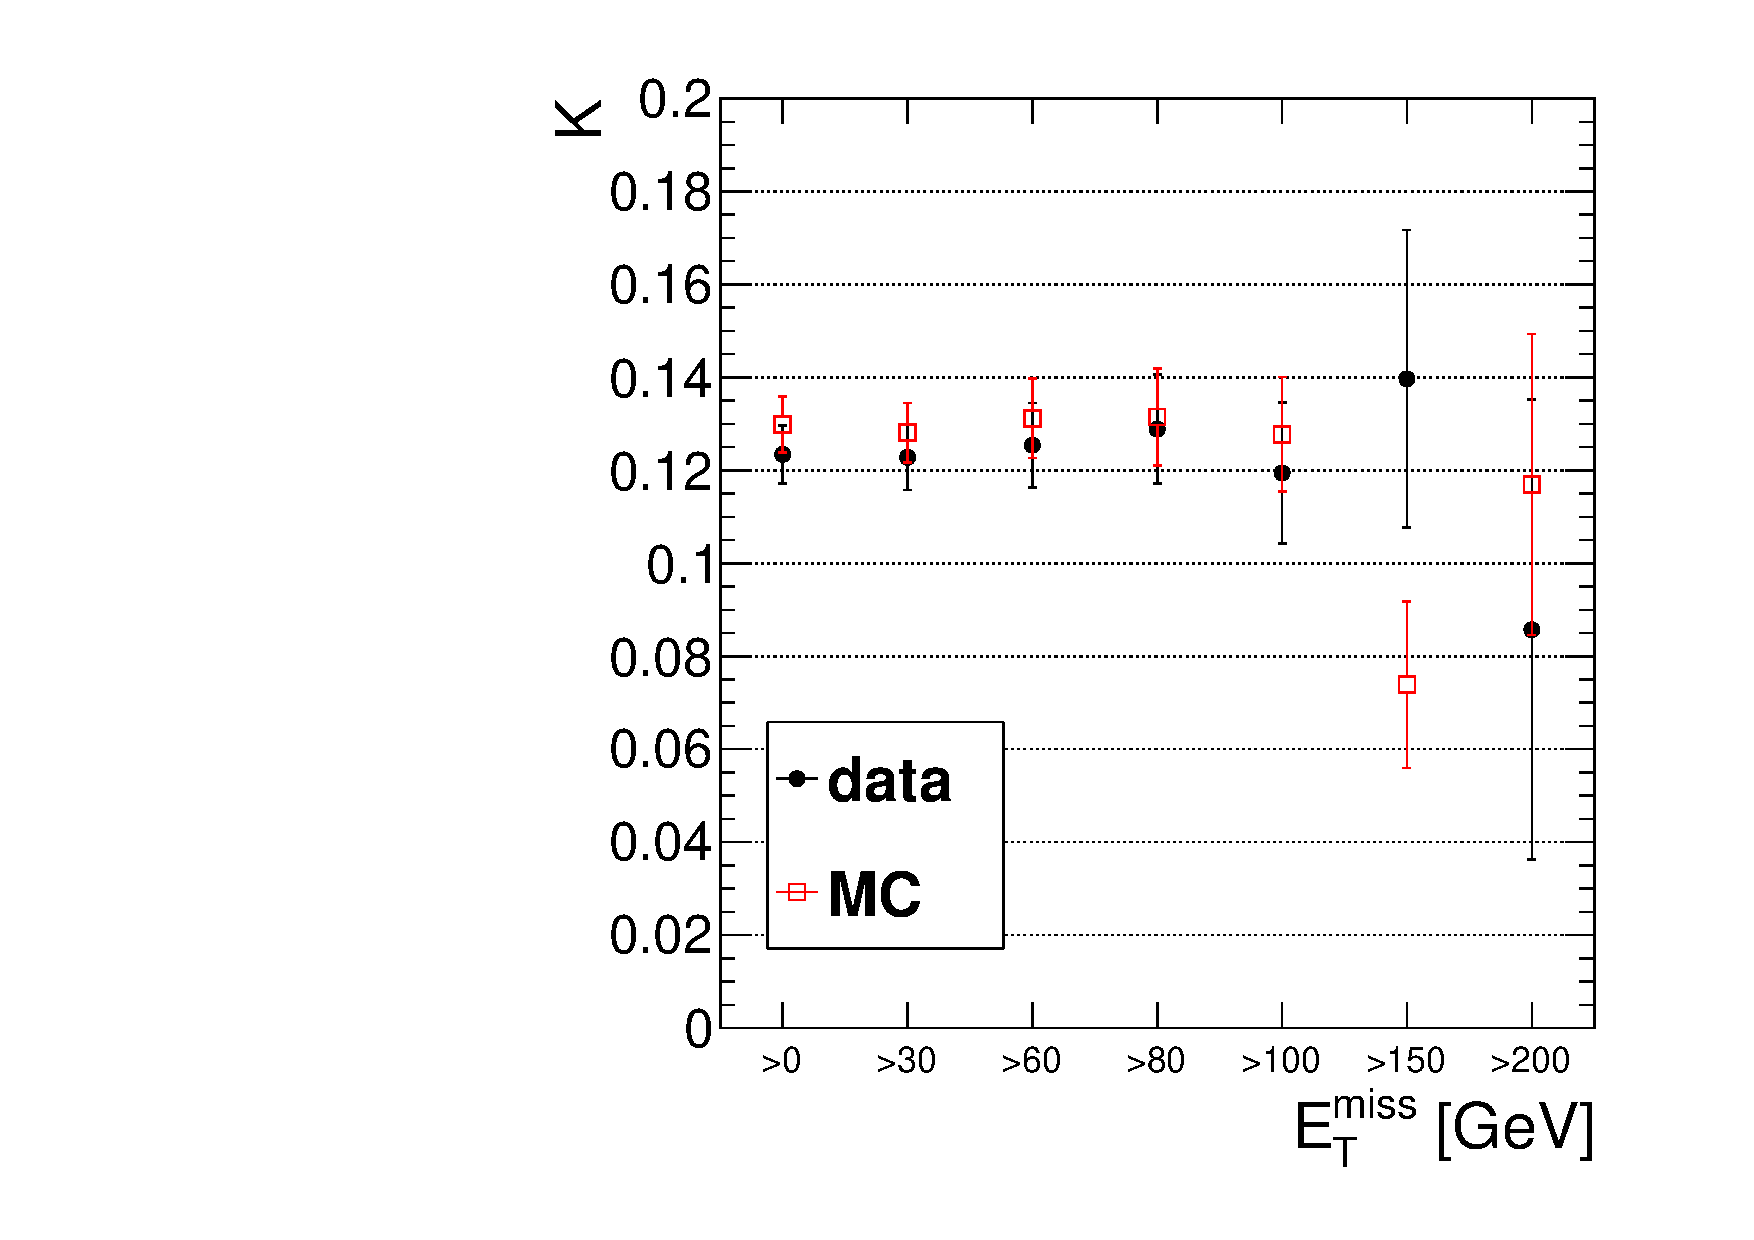
\includegraphics[width=0.4\textwidth]{plots/extractK_inclusive_bveto.pdf} &
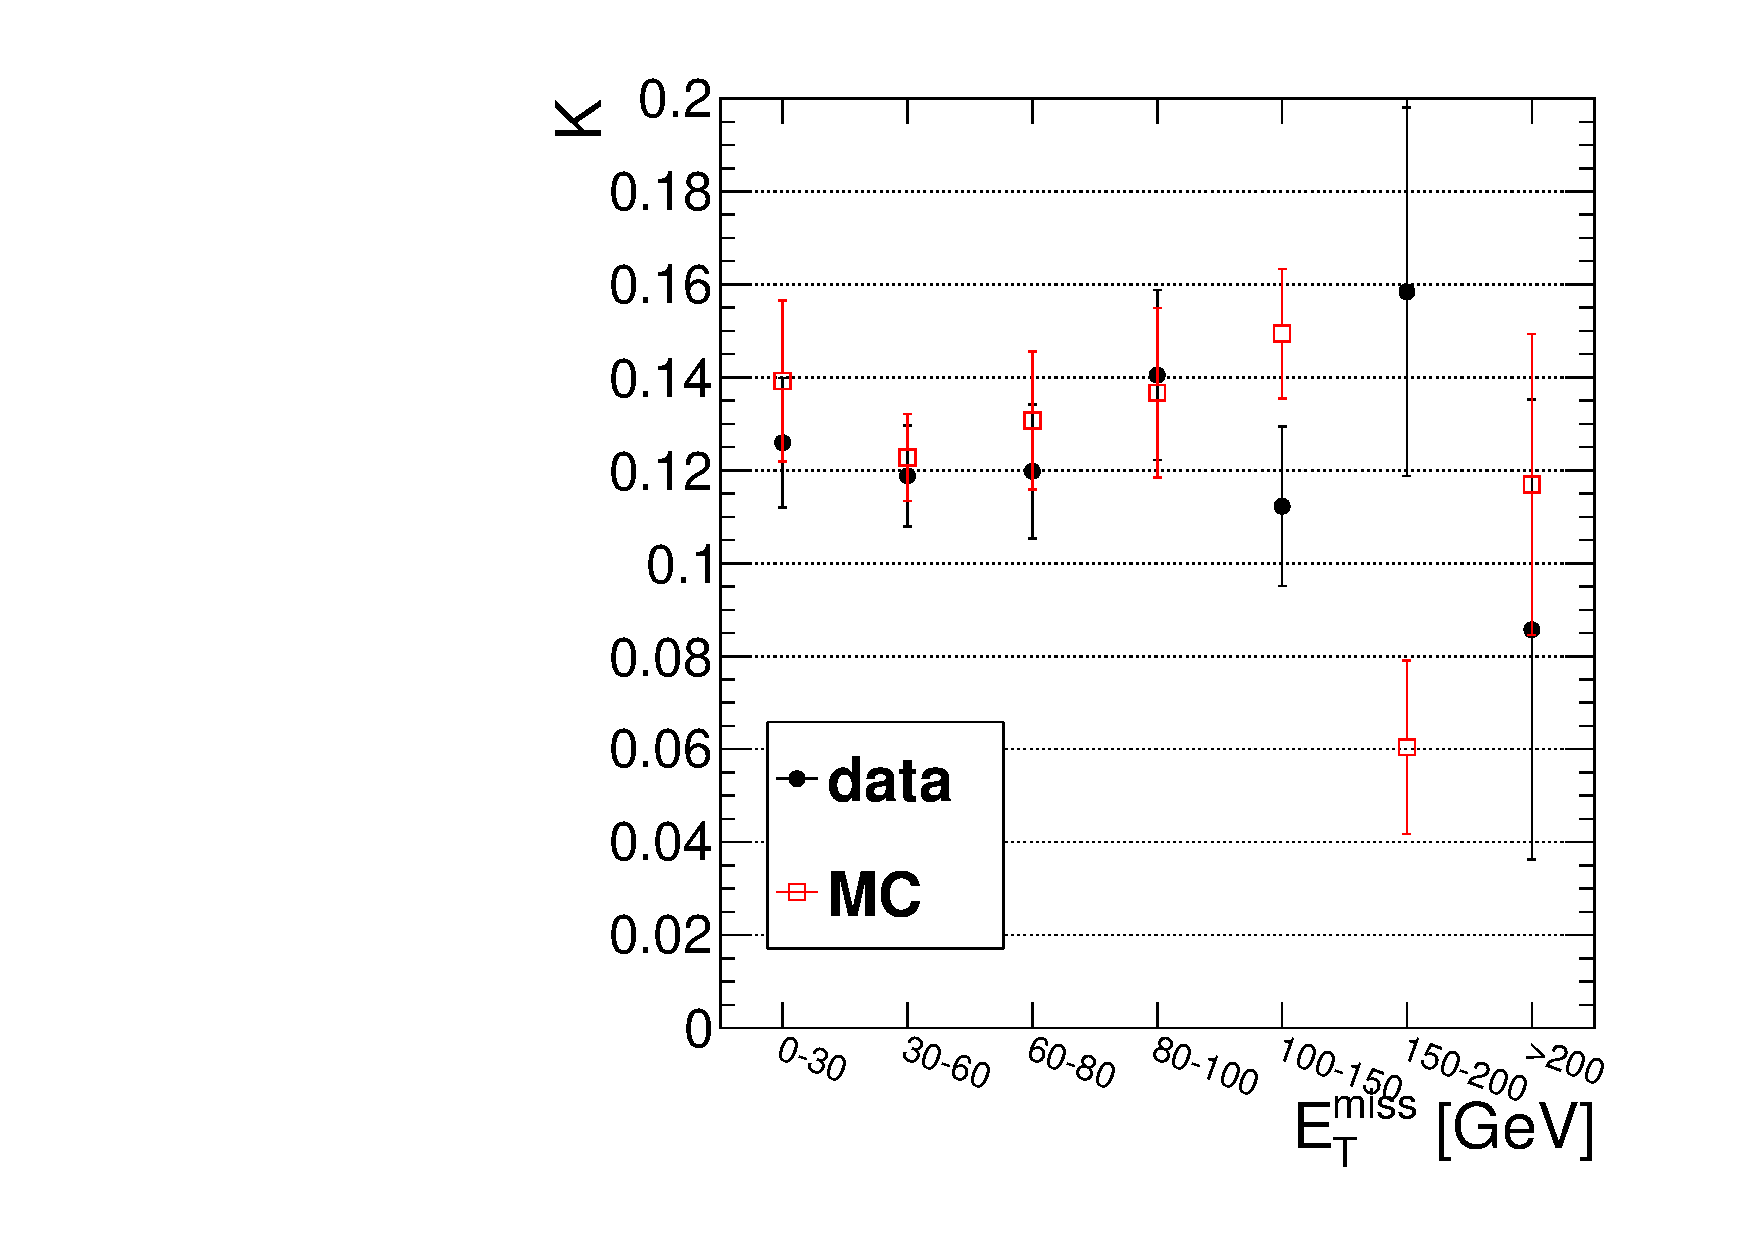
\includegraphics[width=0.4\textwidth]{plots/extractK_exclusive_bveto.pdf} \\
\end{tabular}
\caption{
The efficiency for e$\mu$ events to satisfy the dilepton mass requirement, $K$, in data and simulation for inclusive \MET\ intervals (left) and
exclusive \MET\ intervals (right) for the targeted analysis, including the b-veto. 
Based on this we chose $K=0.13\pm0.02$ for the \MET\ regions up to \MET\ $>$ 100 GeV.
For higher \MET\ regions we chose $K=0.13\pm0.07$.
%{\bf FIXME plots made with 10\% of \zjets\ MC statistics, to be remade with full statistics}
\label{fig:K_targeted}
}
\end{center}
\end{figure}

\clearpage

\subsection{Estimating the WZ and ZZ Background with MC}
\label{sec:bkg_vz}

Backgrounds from W($\ell\nu$)Z($\ell\ell$) where the W lepton is not identified or is outside acceptance, and Z($\nu\nu$)Z($\ell\ell$),
are estimated from simulation. The MC modeling of these processes is validated by comparing the MC predictions with data in control samples
with exactly 3 leptons (WZ control sample) and exactly 4 leptons (ZZ control sample). 
The relevant WZ and ZZ MC samples are:

\begin{itemize}
\footnotesize{
\item \verb=/WZJetsTo3LNu_TuneZ2_8TeV-madgraph-tauola/Summer12-PU_S7_START52_V9-v2/AODSIM= ($\sigma=1.058$ pb),
\item \verb=/ZZJetsTo4L_TuneZ2star_8TeV-madgraph-tauola/Summer12-PU_S7_START52_V9-v3/AODSIM= ($\sigma=0.093$ pb),
}
\end{itemize}
The WZJetsTo2L2Q, ZZJetsTo2L2Q, and ZZJetsTo2L2Nu samples are also used in this analysis but their contribution to the 3-lepton and 4-lepton
control samples is negligible.

\subsubsection{WZ Validation Studies}
\label{sec:bkg_wz}

A pure WZ sample can be selected in data with the requirements:

\begin{itemize}
\item Exactly 3 $p_T>20$~GeV leptons passing analysis identication and isolation requirements,
\item 2 of the 3 leptons must fall in the Z window 81-101 GeV,
\item \MET $>$ 50 GeV (to suppress DY).
\end{itemize}

The data and MC yields passing the above selection are in Table~\ref{tab:wz}. 
The inclusive yields (without any jet requirements) agree within 17\%, which is approximately equal
to the uncertainty in the measured WZ cross section. A data vs. MC comparison of kinematic
distributions (jet multiplicity, \MET, Z \pt) is given in Fig.~\ref{fig:wz}. High \MET\ 
values in WZ and ZZ events arise from highly boosted W or Z bosons that decay leptonically, 
and we therefore check that the MC does a reasonable job of reproducing the \pt distributions of the 
leptonically decaying \Z. While the inclusive WZ yields are in reasonable agreement, we observe
an excess in data in events with at least 2 jets, corresponding to the jet multiplicity requirement
in our preselection. We observe 60 events in data while the MC predicts $34\pm5.2$~(stat), representing an excess of 78\%,
as indicated in Table~\ref{tab:wz2j}. We note some possible contributions to this discrepancy:

\begin{itemize}

\item The \zjets\ contribution is under-estimated here, for 2 reasons: first, because the \zjets\
yield passing a \MET $>$ 50 GeV requirement is under-estimated in MC and second, because the fake
rate is typically under-estimated in the MC. To get a rough idea for how much the excess depends
on the \zjets\ yield, if the \zjets\ yield is doubled then the excess is reduced from 78\% to 55\%.
Also note that we are currently using 10\% of the \zjets\ MC sample and there is 1 event with a weight 
of about 5, so the plots and tables will be remade with full \zjets\ sample.

\item The \ttbar\ contribution is under-estimated here because the fake
rate is typically under-estimated in the MC. To get a rough idea for how much the excess depends
on the \ttbar\ yield, if the \ttbar\ yield is doubled then the excess is reduced from 78\% to 57\%.

\item Currently no attempt is made to reject jets from pile-up interactions, which may be responsible
for some of the excess at large \njets. To check this, we increase the jet \pt threhsold to 40 GeV, which
helps to suppress PU jets, and observe 39 events in data vs. an MC prediction of $25\pm5.2$~(stat),
decreasing the excess from 78\% to 58\%. In the future this may be improved by explicitly
requiring the jets to be consistent with originating from the signal primary vertex.

\end{itemize}

Based on these studies we currently assess an uncertainty of 80\% on the WZ yield.

\begin{table}[htb]
\begin{center}
\caption{\label{tab:wz} Data and Monte Carlo yields passing the WZ preselection. }
\begin{tabular}{lccccc}
\hline
\hline
         Sample   &            ee    &        $\mu\mu$   &        e$\mu$   &          total  \\
\hline
             WZ   & 58.9 $\pm$ 0.7   & 82.2 $\pm$ 0.8   &  4.0 $\pm$ 0.2   &145.1 $\pm$ 1.0  \\
         \ttbar   &  0.6 $\pm$ 0.5   &  4.3 $\pm$ 1.5   &  3.0 $\pm$ 1.2   &  8.0 $\pm$ 2.0  \\
         \zjets   &  0.4 $\pm$ 0.4   &  4.9 $\pm$ 4.9   &  0.0 $\pm$ 0.0   &  5.3 $\pm$ 4.9  \\
             ZZ   &  1.4 $\pm$ 0.0   &  2.0 $\pm$ 0.0   &  0.1 $\pm$ 0.0   &  3.5 $\pm$ 0.0  \\
             WW   &  0.0 $\pm$ 0.0   &  0.2 $\pm$ 0.1   &  0.2 $\pm$ 0.1   &  0.3 $\pm$ 0.1  \\
     single top   &  0.0 $\pm$ 0.0   &  0.0 $\pm$ 0.0   &  0.0 $\pm$ 0.0   &  0.1 $\pm$ 0.1  \\
\hline
    total SM MC   & 61.3 $\pm$ 0.9   & 93.7 $\pm$ 5.2   &  7.3 $\pm$ 1.3   &162.3 $\pm$ 5.4  \\
           data   &             68   &            108   &             14   &            190  \\
\hline
\hline

\end{tabular}
\end{center}
\end{table}

\begin{table}[htb]
\begin{center}
\caption{\label{tab:wz2j} Data and Monte Carlo yields passing the WZ preselection and \njets\ $>$ 2. }
\begin{tabular}{lccccc}
\hline
\hline
         Sample   &            ee    &        $\mu\mu$   &        e$\mu$   &          total  \\
\hline
             WZ   &  9.8 $\pm$ 0.3   & 13.3 $\pm$ 0.3   &  0.6 $\pm$ 0.1   & 23.6 $\pm$ 0.4  \\
         \ttbar   &  0.2 $\pm$ 0.2   &  2.0 $\pm$ 0.9   &  2.2 $\pm$ 1.2   &  4.4 $\pm$ 1.5  \\
         \zjets   &  0.0 $\pm$ 0.0   &  4.9 $\pm$ 4.9   &  0.0 $\pm$ 0.0   &  4.9 $\pm$ 4.9  \\
             ZZ   &  0.3 $\pm$ 0.0   &  0.4 $\pm$ 0.0   &  0.0 $\pm$ 0.0   &  0.7 $\pm$ 0.0  \\
             WW   &  0.0 $\pm$ 0.0   &  0.0 $\pm$ 0.0   &  0.0 $\pm$ 0.0   &  0.1 $\pm$ 0.0  \\
     single top   &  0.0 $\pm$ 0.0   &  0.0 $\pm$ 0.0   &  0.0 $\pm$ 0.0   &  0.0 $\pm$ 0.0  \\
\hline
    total SM MC   & 10.3 $\pm$ 0.3   & 20.8 $\pm$ 5.0   &  2.8 $\pm$ 1.2   & 33.8 $\pm$ 5.2  \\
           data   &             23   &             32   &              5   &             60  \\
\hline
\hline

\end{tabular}
\end{center}
\end{table}

\begin{figure}[tbh]
\begin{center}
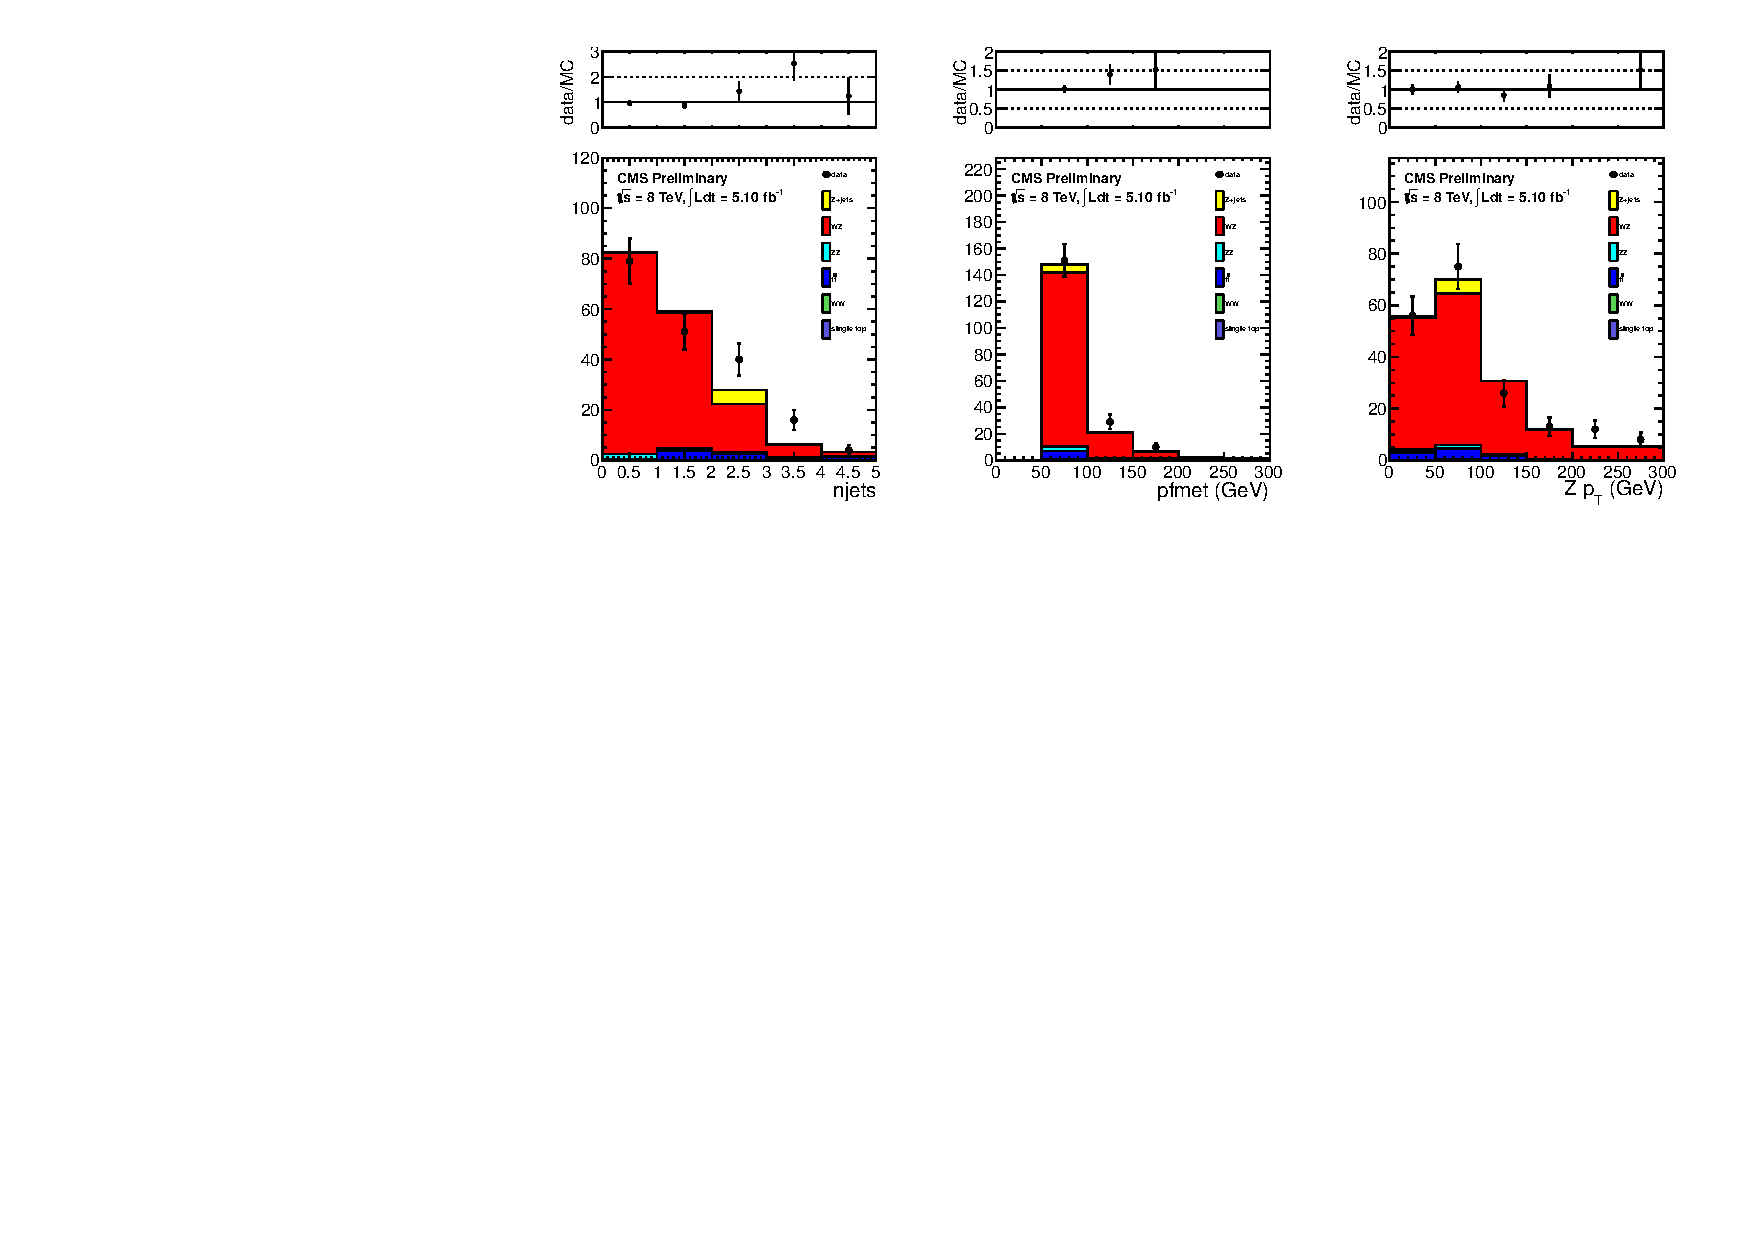
\includegraphics[width=1\linewidth]{plots/WZ.pdf}
\caption{\label{fig:wz}\protect 
Data vs. MC comparisons for the WZ selection discussed in the text for \lumi. 
The number of jets, missing transverse energy, and Z boson transverse momentum are displayed.
}
\end{center}
\end{figure}

\clearpage

\subsubsection{ZZ Validation Studies}
\label{sec:bkg_zz}

A pure ZZ sample can be selected in data with the requirements:

\begin{itemize}
\item Exactly 4 $p_T>20$~GeV leptons passing analysis identication and isolation requirements,
\item 2 of the 4 leptons must fall in the $Z$ window 81-101 GeV.
\end{itemize}

The data and MC yields passing the above selection are in Table~\ref{tab:zz}. Again we observe an
excess in data with respect to the MC prediction (29 observed vs. $17.3\pm0.1$~(stat) MC predicted).
After requiring at least 2 jets, we observe 2 events and the MC predicts $1.5\pm0.1$~(stat).
However, we have recently discovered that we may be using the wrong (too small) cross section for the ZZ sample,
and we are in contact with the MC generator group to determine the correct cross section.
Based on this we currently apply an uncertainty of 80\% to the ZZ background.

\begin{table}[htb]
\begin{center}
\caption{\label{tab:zz} Data and Monte Carlo yields for the ZZ preselection. }
\begin{tabular}{lccccc}
\hline
\hline
         Sample   &             ee   &       $\mu\mu$   &         e$\mu$   &          total  \\
\hline
             ZZ   &  6.6 $\pm$ 0.0   &  9.9 $\pm$ 0.0   &  0.4 $\pm$ 0.0   & 17.0 $\pm$ 0.1  \\
             WZ   &  0.1 $\pm$ 0.0   &  0.2 $\pm$ 0.0   &  0.0 $\pm$ 0.0   &  0.3 $\pm$ 0.0  \\
         \zjets   &  0.0 $\pm$ 0.0   &  0.0 $\pm$ 0.0   &  0.0 $\pm$ 0.0   &  0.0 $\pm$ 0.0  \\
         \ttbar   &  0.0 $\pm$ 0.0   &  0.0 $\pm$ 0.0   &  0.0 $\pm$ 0.0   &  0.0 $\pm$ 0.0  \\
             WW   &  0.0 $\pm$ 0.0   &  0.0 $\pm$ 0.0   &  0.0 $\pm$ 0.0   &  0.0 $\pm$ 0.0  \\
     single top   &  0.0 $\pm$ 0.0   &  0.0 $\pm$ 0.0   &  0.0 $\pm$ 0.0   &  0.0 $\pm$ 0.0  \\
\hline
    total SM MC   &  6.7 $\pm$ 0.0   & 10.1 $\pm$ 0.1   &  0.5 $\pm$ 0.0   & 17.3 $\pm$ 0.1  \\
           data   &             13   &             16   &              0   &             29  \\
\hline
\hline
\end{tabular}
\end{center}
\end{table}

\begin{figure}[tbh]
\begin{center}
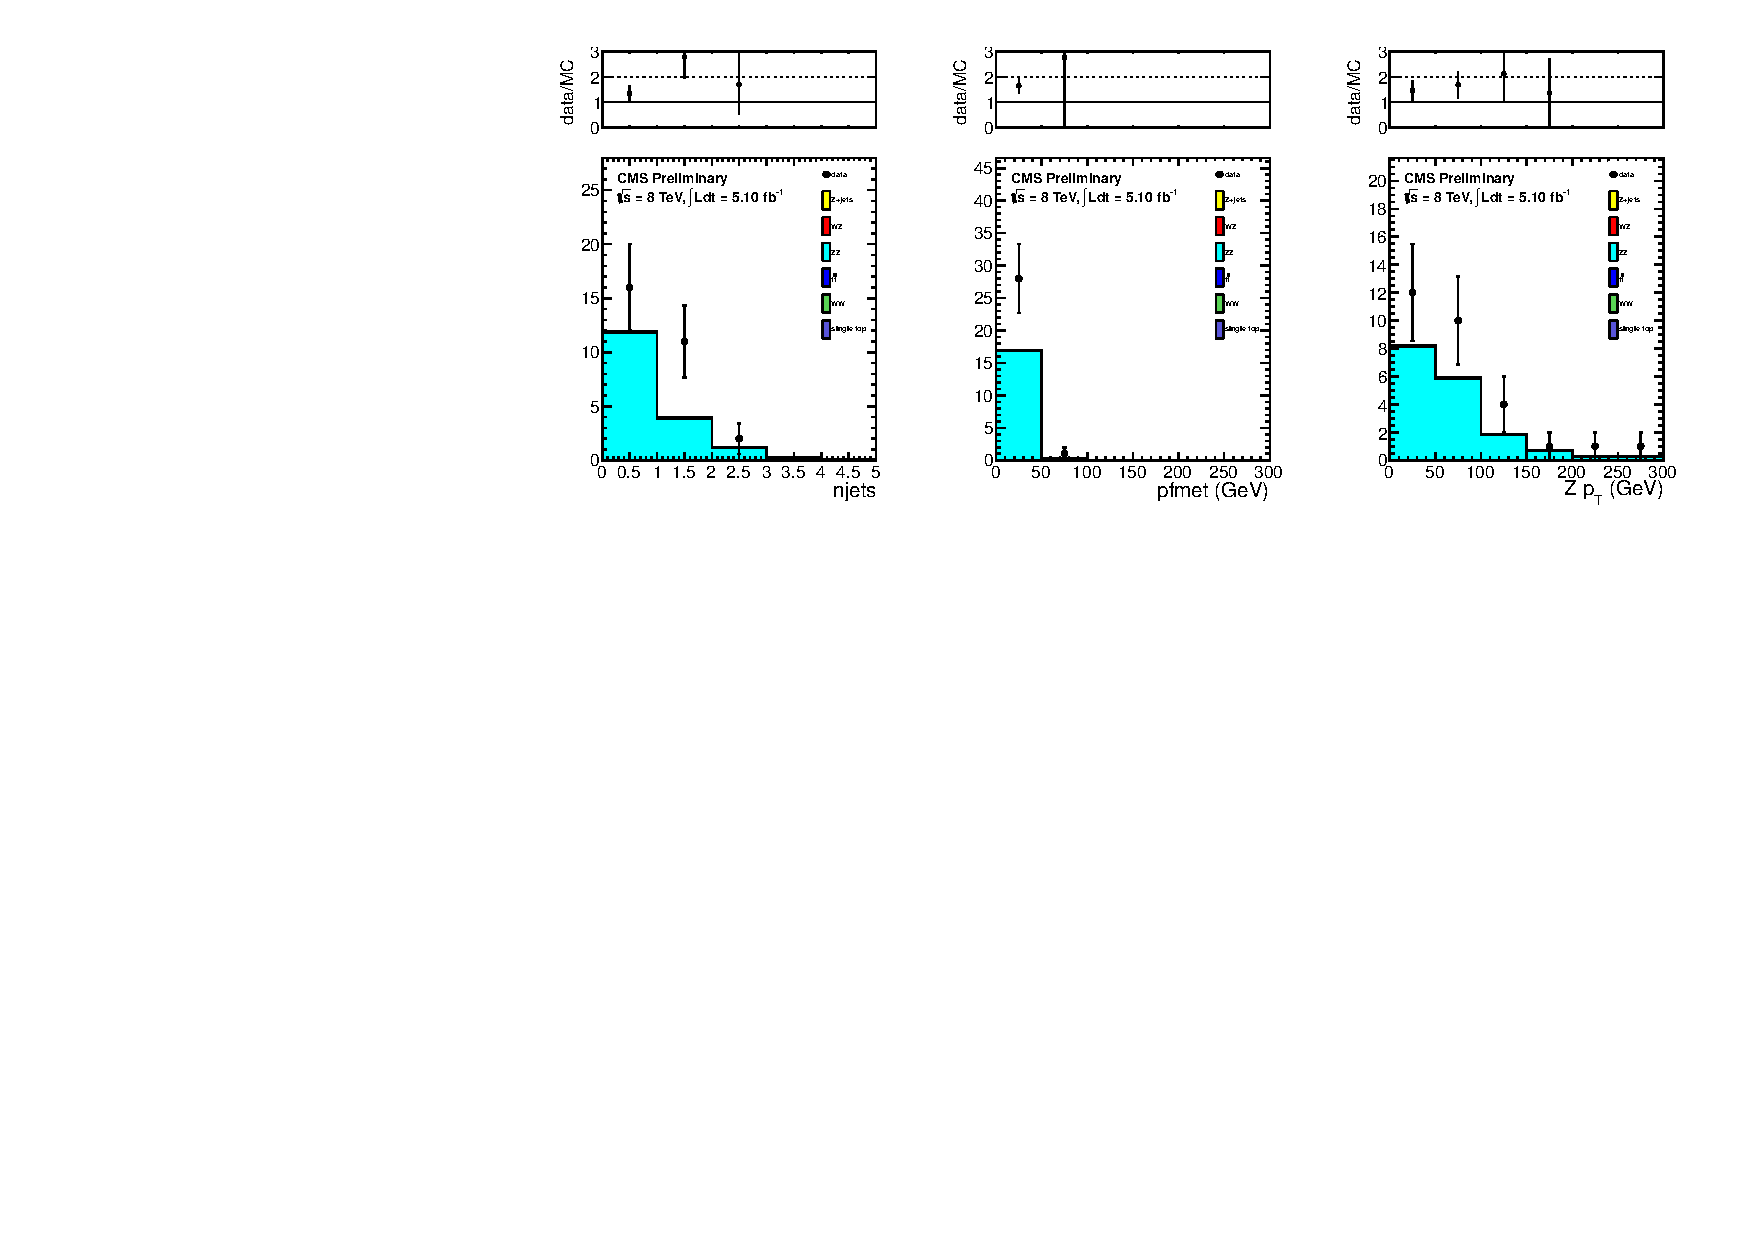
\includegraphics[width=1\linewidth]{plots/ZZ.pdf}
\caption{\label{fig:zz}\protect 
Data vs. MC comparisons for the ZZ selection discussed in the text for \lumi.
The number of jets, missing transverse energy, and Z boson transverse momentum are displayed.
}
\end{center}
\end{figure}




%\subsection{Estimating the Rare SM Backgrounds with MC}
%\label{sec:bkg_raresm}

%{\bf TODO: list samples, yields in preselection region, and show \MET\ distribution}
